\section{TÍCH CỦA VECTƠ VỚI MỘT SỐ THỰC}
\subsection{TÓM TẮT LÝ THUYẾT}
\subsubsection{Định nghĩa}
Cho số thực $k \ne 0$ và $\overrightarrow{a} \ne \vec{0}$.
\begin{center}
	\begin{minipage}[b]{8cm}
		\begin{tcolorbox}[colframe=orange,colback=white,boxrule=0.2mm]
			Tích của vec tơ $\overrightarrow{a}$ với số thực $k>0$ là một vec tơ, kí hiệu $k\overrightarrow{a}$, \indamm{cùng hướng} với $\overrightarrow{a}$ và có đồ dài bằng $k \big|\vec{a}\big|$
		\end{tcolorbox}
	\end{minipage}\hspace{1cm}
	\begin{minipage}[b]{8cm}
		\begin{tcolorbox}[colframe=orange,colback=white,boxrule=0.2mm]
			Tích của vec tơ $\overrightarrow{a}$ với số thực $k<0$ là một vec tơ, kí hiệu $k\overrightarrow{a}$, \indamm{ngược hướng} với $\overrightarrow{a}$ và có đồ dài bằng $\big|k\big|\cdot \big|\vec{a}\big|$
		\end{tcolorbox}
	\end{minipage}
\end{center}
\immini{\indamm{ Ví dụ:} Theo hình vẽ bên, thì $\overrightarrow{b}=3\overrightarrow{a}$; $\overrightarrow{c}=-2\overrightarrow{a}$; $\overrightarrow{c}=-\dfrac{2}{3}\overrightarrow{b}$.
	\begin{luuy}
		Quy ước: $0 \cdot \overrightarrow{a}=\overrightarrow{0}$.
	\end{luuy}
}{
	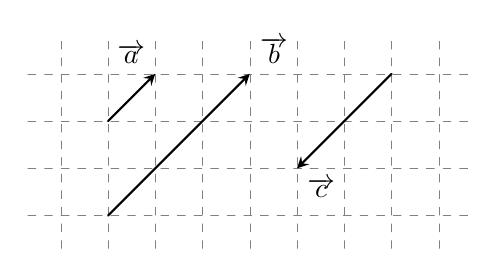
\begin{tikzpicture}[>=stealth,scale=0.6, line join=round, line cap=round]
		\draw[line width=0.05pt,gray,dashed] (-0.7,-0.7) grid (8.7,3.7);
		\draw[->,thick](1,2)--(2,3)node[above left]{$\overrightarrow{a}$};
		\draw[->,thick](1,0)--(4,3)node[above right]{$\overrightarrow{b}$};
		\draw[->,thick](7,3)--(5,1)node[below right]{$\overrightarrow{c}$};
\end{tikzpicture}}

\subsubsection{Điều kiện để hai vectơ cùng phương}
\begin{gachsoc}
	\begin{itemize}
		\item [\ding{172}] Điều kiện cần và đủ để $\overrightarrow{a}$ và $\overrightarrow{b} \ne \overrightarrow{0}$ cùng phương là có một số thực $k$ để $\overrightarrow{a}=k\overrightarrow{b}$.
		\item [\ding{173}] Ba điểm phân biệt $A$, $B$, $C$ thẳng hàng khi có số thực $k$ để $\overrightarrow{AB}=k\overrightarrow{AC}$.
	\end{itemize}
\end{gachsoc}
\subsubsection{Tính chất}
\begin{tcolorbox}[colframe=orange,colback=white,boxrule=0.2mm]
	Với hai vec tơ $\vec{a}$, $\vec{b}$ và hai số thực $k$, $t$ ta luôn có
	\begin{listEX}[3]
		\item [$\bullet$] $k(t\vec{a})=(k \cdot t)\vec{a}$.
		\item [$\bullet$] $(k+t)\vec{a}=k\vec{a}+t\vec{a}$.
		\item [$\bullet$] $k(\vec{a}+\vec{b})=k\vec{a}+k\vec{b}$.
		\item [$\bullet$] $k(\vec{a}-\vec{b})=k\vec{a}-k\vec{b}$.
		\item [$\bullet$] $1\cdot \vec{a})=\vec{a}$. 
		\item [$\bullet$] $(-1)\cdot \vec{a})=-\vec{a}$.
	\end{listEX}
\end{tcolorbox}
\subsubsection{Phân tích một vectơ theo hai vectơ không cùng phương}
\begin{gachsoc}
	\immini{Cho hai vectơ $\vec{a}$ và $\vec{b}$ không cùng phương. Khi đó mọi vectơ $\vec{c}$ đều phân tích được một cách duy nhất theo hai vectơ $\vec{a}$ và $\vec{b}$, nghĩa là có duy nhất cặp số $h,k$ sao cho $\vec{c}=h\vec{a}+k\vec{b}$
		\begin{itemize}
			\item [$\bullet$] Theo quy tắc hình bình hành, ta có $$\overrightarrow{c}=\overrightarrow{OH}+\overrightarrow{OK}$$
			\item [$\bullet$] Giả sử $\overrightarrow{OH}= h\overrightarrow{a}$ và $\overrightarrow{OK}= k\overrightarrow{b}$ thì $\vec{c}=h\vec{a}+k\vec{b}$.
		\end{itemize}
	}{
		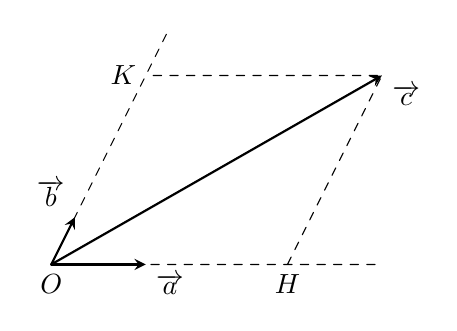
\begin{tikzpicture}[>=stealth,scale=0.6, line join=round, line cap=round]
			%\draw[line width=0.05pt,gray,dashed] (-0.7,-0.7) grid (8.7,4.7);
			\draw[->,thick](0,0)--(0.5,1)node[above left]{$\overrightarrow{b}$};
			\draw[->,thick](0,0)--(2,0)node[below right]{$\overrightarrow{a}$};
			\draw[->,thick](0,0)--(7,4)node[below right]{$\overrightarrow{c}$};
			\draw[dashed](0,0)--(7,0) (0,0)--(2.5,5) (5,0)--(7,4)--(2,4);
			\node[below] at (5,0) {$H$};
			\node[below] at (0,0) {$O$};
			\node[left] at (2,4) {$K$};
	\end{tikzpicture}}
\end{gachsoc}

\subsection{RÈN LUYỆN KĨ NĂNG GIẢI TOÁN}
\begin{dang}{So sánh hai vectơ theo tỉ số $k$ tương ứng}
	\begin{enumerate}[\faPencilSquareO]
		\item Xét hai vec tơ cùng phương $\overrightarrow{AB}$ và $\overrightarrow{CD}$.
		\begin{itemize}
			\item Bước 1. Tính tỉ lệ đoạn thẳng $\dfrac{AB}{CD}=m$.
			\item Bước 2. Xem xét, nếu
			\begin{itemize}
				\item $\overrightarrow{AB}$ cùng hướng với $\overrightarrow{CD}$ thì $\overrightarrow{AB}=m\overrightarrow{CD}$.
				\item $\overrightarrow{AB}$ ngược hướng với $\overrightarrow{CD}$ thì $\overrightarrow{AB}=-m\overrightarrow{CD}$.
			\end{itemize}
		\end{itemize}
	\end{enumerate}
\end{dang}

\begin{vd}
	Cho đoạn thẳng $AB$ và $M$ là trung điểm của đoạn $AB$. Tìm số $k$ trong các đẳng thức sau:
	\begin{enumEX}[a)]{4}
		\item  $\overrightarrow{AB}=k\overrightarrow{MB}$.
		\item  $\overrightarrow{MA}=k\overrightarrow{MB}$.
		\item $\overrightarrow{MA}=k\overrightarrow{AB}$.
		\item $\overrightarrow{MB}=k\overrightarrow{AB}$.
	\end{enumEX}
	\loigiai{
	Vì $M$ là trung điểm của đoạn thẳng $AB$ nên $AB = 2MB = 2MA$.
	\begin{enumerate}
		\item[a)] Hai vectơ $\overrightarrow{AB}$ và $\overrightarrow{MB}$ ngược hướng và $|\overrightarrow{AB}| = 2|\overrightarrow{MB}|$ nên $\overrightarrow{AB} = -2\overrightarrow{MB}$. Vậy $k = -2$.
		\item[b)] Hai vectơ $\overrightarrow{MA}$ và $\overrightarrow{MB}$ là hai vectơ đối nhau nên $\overrightarrow{MA} = -\overrightarrow{MB}$. Vậy $k = -1$.
		\item[c)] Hai vectơ $\overrightarrow{MA}$ và $\overrightarrow{AB}$ ngược hướng và $|\overrightarrow{MA}| = \dfrac{1}{2}|\overrightarrow{AB}|$ nên $\overrightarrow{MA} = -\dfrac{1}{2}\overrightarrow{AB}$. Vậy $k = -\dfrac{1}{2}$.
		\item[d)] Hai vectơ $\overrightarrow{MB}$ và $\overrightarrow{AB}$ cùng hướng và $|\overrightarrow{MB}| = \dfrac{1}{2}|\overrightarrow{AB}|$ nên $\overrightarrow{MB} = \dfrac{1}{2}\overrightarrow{AB}$. Vậy $k = \dfrac{1}{2}$.
	\end{enumerate}
}
\end{vd}
\dongcham{2}
\begin{vd}
	Cho tam giác $ABC$ có trọng tâm $G$. Gọi $M$ là trung điểm của $BC$. Tìm số $k$ trong các đẳng thức sau:
	\begin{enumEX}[a)]{4}
		\item $\overrightarrow{AG}=k\overrightarrow{MG}$.
		\item $\overrightarrow{AM}=k\overrightarrow{GA}$.
		\item $\overrightarrow{GM}=k\overrightarrow{GA}$.
		\item $\overrightarrow{GM}=k\overrightarrow{AM}$.
	\end{enumEX}
	\loigiai{
	Vì $G$ là trọng tâm của tam giác $ABC$ và $AM$ là đường trung tuyến nên $A, G, M$ thẳng hàng, $G$ nằm giữa $A$ và $M$, đồng thời $AG = 2GM = \dfrac{2}{3}AM$.
	\begin{enumerate}
		\item[a)] $\overrightarrow{AG}$ và $\overrightarrow{MG}$ ngược hướng, $AG = 2MG \Rightarrow \overrightarrow{AG} = -2\overrightarrow{MG}$. Vậy $k = -2$.
		\item[b)] $\overrightarrow{AM}$ và $\overrightarrow{GA}$ ngược hướng. Ta có $AM = \dfrac{3}{2}AG = \dfrac{3}{2}GA \Rightarrow \overrightarrow{AM} = -\dfrac{3}{2}\overrightarrow{GA}$. Vậy $k = -\dfrac{3}{2}$.
		\item[c)] $\overrightarrow{GM}$ và $\overrightarrow{GA}$ cùng hướng, $GM = \dfrac{1}{2}GA \Rightarrow \overrightarrow{GM} = \dfrac{1}{2}\overrightarrow{GA}$ (Lưu ý: $\overrightarrow{GM}$ và $\overrightarrow{GA}$ thực chất cùng hướng vì $G$ nằm giữa $A$ và $M$... Khoan, $G$ nằm giữa $A$ và $M$ nên tia $GM$ và tia $GA$ ngược hướng! Xin lỗi, $\overrightarrow{GM}$ và $\overrightarrow{GA}$ ngược hướng). Suy ra $\overrightarrow{GM} = -\dfrac{1}{2}\overrightarrow{GA}$. Vậy $k = -\dfrac{1}{2}$.
		\item[d)] $\overrightarrow{GM}$ và $\overrightarrow{AM}$ cùng hướng, $GM = \dfrac{1}{3}AM \Rightarrow \overrightarrow{GM} = \dfrac{1}{3}\overrightarrow{AM}$. Vậy $k = \dfrac{1}{3}$.
	\end{enumerate}
}
\end{vd}
\dongcham{2}
\begin{dang}{Chứng minh đẳng thức vectơ}
	
\end{dang}

\begin{vd}
	Cho hình bình hành $ABCD$ tâm $O$. Gọi $G$ là trọng tâm tam giác $ABC$. Chứng minh
	\begin{tasks}(2)
		\task $\overrightarrow{AB}+\overrightarrow{AD}=2\overrightarrow{AO}$;
		\task $\overrightarrow{AB}+\overrightarrow{AC}+\overrightarrow{AD}=2\overrightarrow{AC}$;
		\task $\overrightarrow{AB}+\overrightarrow{OD}-\dfrac{1}{2}\overrightarrow{AC}=\overrightarrow{0}$;
		\task $\overrightarrow{GA}+\overrightarrow{GC}=\dfrac{1}{3}\overrightarrow{BD}$.
	\end{tasks}
	\loigiai{
	\begin{enumerate}
		\item[a)] Theo quy tắc hình bình hành, $\overrightarrow{AB} + \overrightarrow{AD} = \overrightarrow{AC}$. Mà $O$ là trung điểm $AC$ nên $\overrightarrow{AC} = 2\overrightarrow{AO}$. Suy ra $\overrightarrow{AB} + \overrightarrow{AD} = 2\overrightarrow{AO}$.
		\item[b)] Ta có $VT = (\overrightarrow{AB} + \overrightarrow{AD}) + \overrightarrow{AC} = \overrightarrow{AC} + \overrightarrow{AC} = 2\overrightarrow{AC} = VP$.
		\item[c)] Vì $O$ là trung điểm $AC$ nên $\dfrac{1}{2}\overrightarrow{AC} = \overrightarrow{AO}$. Thay vào vế trái:
		$$ VT = \overrightarrow{AB} + \overrightarrow{OD} - \overrightarrow{AO} = \overrightarrow{AB} + \overrightarrow{OA} + \overrightarrow{OD} = (\overrightarrow{OA} + \overrightarrow{AB}) + \overrightarrow{OD} = \overrightarrow{OB} + \overrightarrow{OD} $$
		Do $O$ là trung điểm $BD$ nên $\overrightarrow{OB} + \overrightarrow{OD} = \vec{0}$. Suy ra $VT = \vec{0} = VP$.
		\item[d)] Vì $O$ là trung điểm $AC$ nên $\overrightarrow{GA} + \overrightarrow{GC} = 2\overrightarrow{GO}$.\\
		Trong tam giác $ABC$, $BO$ là đường trung tuyến và $G$ là trọng tâm nên $\overrightarrow{GO} = \dfrac{1}{3}\overrightarrow{BO}$.\\
		Mặt khác, do $O$ là trung điểm $BD$ nên $\overrightarrow{BO} = \dfrac{1}{2}\overrightarrow{BD}$.\\
		Thay vào ta được: $2\overrightarrow{GO} = 2 \cdot \dfrac{1}{3}\overrightarrow{BO} = \dfrac{2}{3} \cdot \dfrac{1}{2}\overrightarrow{BD} = \dfrac{1}{3}\overrightarrow{BD}$ (đpcm).
	\end{enumerate}
}
\end{vd} \dongcham{12}

\begin{vd}
	Cho hình bình hành $ABCD$ có tâm $O$, $M$ là điểm bất kì trong mặt phẳng. Chứng minh rằng
	\begin{tasks}(2)
		\task $\overrightarrow{OA}+\overrightarrow{OB}+\overrightarrow{OC}+\overrightarrow{OD}=\overrightarrow{0}$;
		\task $\overrightarrow{MA}+\overrightarrow{MB}+\overrightarrow{MC}+\overrightarrow{MD}=4\overrightarrow{MO}$.
	\end{tasks}
	\loigiai{
	\begin{enumerate}
		\item[a)] Vì $O$ là tâm hình bình hành nên $O$ là trung điểm của $AC$ và $BD$. Suy ra $\overrightarrow{OA} + \overrightarrow{OC} = \vec{0}$ và $\overrightarrow{OB} + \overrightarrow{OD} = \vec{0}$.\\
		Do đó: $VT = (\overrightarrow{OA} + \overrightarrow{OC}) + (\overrightarrow{OB} + \overrightarrow{OD}) = \vec{0} + \vec{0} = \vec{0} = VP$.
		\item[b)] Theo quy tắc chèn điểm $O$, ta có:
		$$ VT = (\overrightarrow{MO} + \overrightarrow{OA}) + (\overrightarrow{MO} + \overrightarrow{OB}) + (\overrightarrow{MO} + \overrightarrow{OC}) + (\overrightarrow{MO} + \overrightarrow{OD}) $$
		$$ VT = 4\overrightarrow{MO} + (\overrightarrow{OA} + \overrightarrow{OB} + \overrightarrow{OC} + \overrightarrow{OD}) $$
		Áp dụng kết quả câu a, ta được: $VT = 4\overrightarrow{MO} + \vec{0} = 4\overrightarrow{MO} = VP$.
	\end{enumerate}
}
\end{vd} \dongcham{13}

\begin{vd}
	Cho tam giác $ABC$ Gọi $M$ là trung điểm $BC$, $D$ là trung điểm $AM$; $O$ là điểm bất kì trong mặt phẳng. Chứng minh rằng
	\begin{tasks}(2)
		\task $\overrightarrow{AB}+\overrightarrow{AC}=2\overrightarrow{AM}$;
		\task $\overrightarrow{BA}+\overrightarrow{BM}+2\overrightarrow{DB}=\overrightarrow{0}$;
		\task $2\overrightarrow{DA}+\overrightarrow{DB}+\overrightarrow{DC}=\overrightarrow{0}$;
		\task $2\overrightarrow{OA}+\overrightarrow{OB}+\overrightarrow{OC}=4\overrightarrow{OD}$.
	\end{tasks}
	\loigiai{
	\begin{enumerate}
		\item[a)] Do $M$ là trung điểm của $BC$ nên áp dụng quy tắc trung điểm ta có ngay $\overrightarrow{AB} + \overrightarrow{AC} = 2\overrightarrow{AM}$.
		\item[b)] Áp dụng quy tắc trung điểm cho tam giác $ABM$ với $D$ là trung điểm cạnh $AM$, ta có $\overrightarrow{BA} + \overrightarrow{BM} = 2\overrightarrow{BD}$.
		Thay vào vế trái: $VT = 2\overrightarrow{BD} + 2\overrightarrow{DB} = 2(\overrightarrow{BD} + \overrightarrow{DB}) = 2\vec{0} = \vec{0} = VP$.
		\item[c)] Vì $M$ là trung điểm $BC$ nên $\overrightarrow{DB} + \overrightarrow{DC} = 2\overrightarrow{DM}$.
		Thay vào vế trái: $VT = 2\overrightarrow{DA} + 2\overrightarrow{DM} = 2(\overrightarrow{DA} + \overrightarrow{DM})$.
		Do $D$ là trung điểm $AM$ nên $\overrightarrow{DA} + \overrightarrow{DM} = \vec{0}$. Suy ra $VT = \vec{0} = VP$.
		\item[d)] Chèn điểm $O$ vào biểu thức ở câu c, ta có:
		$$ 2(\overrightarrow{OA} - \overrightarrow{OD}) + (\overrightarrow{OB} - \overrightarrow{OD}) + (\overrightarrow{OC} - \overrightarrow{OD}) = \vec{0} $$
		$$ \Leftrightarrow 2\overrightarrow{OA} + \overrightarrow{OB} + \overrightarrow{OC} - 4\overrightarrow{OD} = \vec{0} $$
		$$ \Leftrightarrow 2\overrightarrow{OA} + \overrightarrow{OB} + \overrightarrow{OC} = 4\overrightarrow{OD} \text{ (đpcm)}. $$
	\end{enumerate}
}
\end{vd} \dongcham{21}

\begin{vd}
	Cho tứ giác $ABCD$. Gọi $I$, $J $ lần lượt là trung điểm $AB$, $CD$. Chứng minh
	\begin{tasks}(2)
		\task $2\overrightarrow{IJ}=\overrightarrow{AC}+\overrightarrow{BD}=\overrightarrow{AD}+\overrightarrow{BC}$ ;
		\task $\overrightarrow{AD}+\overrightarrow{BD}+\overrightarrow{AC}+\overrightarrow{BC}=4\overrightarrow{IJ}$.
	\end{tasks}
	\loigiai{
	\begin{enumerate}
		\item[a)] Áp dụng quy tắc chèn điểm $I$ và $J$:
		$$ \overrightarrow{AC} + \overrightarrow{BD} = (\overrightarrow{AI} + \overrightarrow{IJ} + \overrightarrow{JC}) + (\overrightarrow{BI} + \overrightarrow{IJ} + \overrightarrow{JD}) $$
		$$ = 2\overrightarrow{IJ} + (\overrightarrow{AI} + \overrightarrow{BI}) + (\overrightarrow{JC} + \overrightarrow{JD}) $$
		Vì $I, J$ lần lượt là trung điểm $AB, CD$ nên $\overrightarrow{AI} + \overrightarrow{BI} = \vec{0}$ và $\overrightarrow{JC} + \overrightarrow{JD} = \vec{0}$.\\
		Suy ra $\overrightarrow{AC} + \overrightarrow{BD} = 2\overrightarrow{IJ}$ (1).\\
		Tương tự: $\overrightarrow{AD} + \overrightarrow{BC} = (\overrightarrow{AI} + \overrightarrow{IJ} + \overrightarrow{JD}) + (\overrightarrow{BI} + \overrightarrow{IJ} + \overrightarrow{JC})$
		$$ = 2\overrightarrow{IJ} + (\overrightarrow{AI} + \overrightarrow{BI}) + (\overrightarrow{JD} + \overrightarrow{JC}) = 2\overrightarrow{IJ} \text{ (2)}. $$
		Từ (1) và (2) suy ra $2\overrightarrow{IJ} = \overrightarrow{AC} + \overrightarrow{BD} = \overrightarrow{AD} + \overrightarrow{BC}$.
		\item[b)] Cộng vế theo vế đẳng thức (1) và (2) ở câu a, ta được:
		$$ (\overrightarrow{AC} + \overrightarrow{BD}) + (\overrightarrow{AD} + \overrightarrow{BC}) = 2\overrightarrow{IJ} + 2\overrightarrow{IJ} $$
		$$ \Leftrightarrow \overrightarrow{AD} + \overrightarrow{BD} + \overrightarrow{AC} + \overrightarrow{BC} = 4\overrightarrow{IJ} \text{ (đpcm)}. $$
	\end{enumerate}
}
\end{vd} \dongcham{20}

\begin{vd}
	Cho tứ giác $ABCD$.  Gọi $M$, $N$ lần lượt là trung điểm $AC$, $BD$. Gọi $I$ là trung điểm $MN$. Chứng minh rằng
	\begin{tasks}(2)
		\task $\overrightarrow{IA}+\overrightarrow{IB}+\overrightarrow{IC}+\overrightarrow{ID}=\overrightarrow{0}$;
		\task $\overrightarrow{OA}+\overrightarrow{OB}+\overrightarrow{OC}+\overrightarrow{OD}=4\overrightarrow{OI}$
	\end{tasks}
	\loigiai{
	\begin{enumerate}
		\item[a)] Gộp các vectơ theo từng cặp để sử dụng tính chất trung điểm:
		$$ VT = (\overrightarrow{IA} + \overrightarrow{IC}) + (\overrightarrow{IB} + \overrightarrow{ID}) $$
		Vì $M$ là trung điểm $AC$ nên $\overrightarrow{IA} + \overrightarrow{IC} = 2\overrightarrow{IM}$.\\
		Vì $N$ là trung điểm $BD$ nên $\overrightarrow{IB} + \overrightarrow{ID} = 2\overrightarrow{IN}$.\\
		Suy ra $VT = 2\overrightarrow{IM} + 2\overrightarrow{IN} = 2(\overrightarrow{IM} + \overrightarrow{IN})$.\\
		Mà $I$ là trung điểm $MN$ nên $\overrightarrow{IM} + \overrightarrow{IN} = \vec{0}$. Do đó $VT = \vec{0} = VP$.
		\item[b)] Chèn điểm $I$ vào vế trái của đẳng thức:
		$$ VT = (\overrightarrow{OI} + \overrightarrow{IA}) + (\overrightarrow{OI} + \overrightarrow{IB}) + (\overrightarrow{OI} + \overrightarrow{IC}) + (\overrightarrow{OI} + \overrightarrow{ID}) $$
		$$ VT = 4\overrightarrow{OI} + (\overrightarrow{IA} + \overrightarrow{IB} + \overrightarrow{IC} + \overrightarrow{ID}) $$
		Áp dụng kết quả câu a, ta có $\overrightarrow{IA} + \overrightarrow{IB} + \overrightarrow{IC} + \overrightarrow{ID} = \vec{0}$.\\
		Suy ra $VT = 4\overrightarrow{OI} + \vec{0} = 4\overrightarrow{OI} = VP$.
	\end{enumerate}
}
\end{vd} \dongcham{15}

\begin{vd}
	Cho $\Delta ABC$. Gọi $M,\text{ }N,\text{ }K$ lần lượt là trung điểm cạnh $AB$, $BC$, $CA$; $G$ là trọng tâm tam giác $ABC$. Chứng minh rằng
	\begin{tasks}(2)
		\task $\overrightarrow{AM}+\overrightarrow{BN}+\overrightarrow{CK}=\overrightarrow{0}$;
		\task $\overrightarrow{AK}+\overrightarrow{CN}+\overrightarrow{BM}=\overrightarrow{0}$;
		\task $\overrightarrow{AN}+\overrightarrow{BK}+\overrightarrow{CM}=\overrightarrow{0}$;
		\task $\overrightarrow{GM}+\overrightarrow{GN}+\overrightarrow{GK}=\overrightarrow{0}$.
	\end{tasks}
	\loigiai{
	\begin{enumerate}
		\item[a)] Vì $M, N, K$ là trung điểm các cạnh nên ta có $\overrightarrow{AM} = \dfrac{1}{2}\overrightarrow{AB}$, $\overrightarrow{BN} = \dfrac{1}{2}\overrightarrow{BC}$, $\overrightarrow{CK} = \dfrac{1}{2}\overrightarrow{CA}$.
		$$ VT = \dfrac{1}{2}\overrightarrow{AB} + \dfrac{1}{2}\overrightarrow{BC} + \dfrac{1}{2}\overrightarrow{CA} = \dfrac{1}{2}(\overrightarrow{AB} + \overrightarrow{BC} + \overrightarrow{CA}) = \dfrac{1}{2}(\overrightarrow{AC} + \overrightarrow{CA}) = \vec{0} = VP. $$
		\item[b)] Tương tự câu a, ta có $\overrightarrow{AK} = \dfrac{1}{2}\overrightarrow{AC}$, $\overrightarrow{CN} = \dfrac{1}{2}\overrightarrow{CB}$, $\overrightarrow{BM} = \dfrac{1}{2}\overrightarrow{BA}$.
		$$ VT = \dfrac{1}{2}\overrightarrow{AC} + \dfrac{1}{2}\overrightarrow{CB} + \dfrac{1}{2}\overrightarrow{BA} = \dfrac{1}{2}(\overrightarrow{AB} + \overrightarrow{BA}) = \vec{0} = VP. $$
		\item[c)] Áp dụng công thức đường trung tuyến cho tam giác $ABC$:
		$$ \overrightarrow{AN} = \dfrac{1}{2}(\overrightarrow{AB} + \overrightarrow{AC}); \quad \overrightarrow{BK} = \dfrac{1}{2}(\overrightarrow{BA} + \overrightarrow{BC}); \quad \overrightarrow{CM} = \dfrac{1}{2}(\overrightarrow{CA} + \overrightarrow{CB}) $$
		Cộng vế theo vế:
		$$ VT = \dfrac{1}{2}(\overrightarrow{AB} + \overrightarrow{BA} + \overrightarrow{AC} + \overrightarrow{CA} + \overrightarrow{BC} + \overrightarrow{CB}) = \dfrac{1}{2}(\vec{0} + \vec{0} + \vec{0}) = \vec{0} = VP. $$
		\item[d)] Áp dụng công thức trung điểm cho các đoạn $AB, BC, CA$ với điểm $G$:
		$$ \overrightarrow{GM} = \dfrac{1}{2}(\overrightarrow{GA} + \overrightarrow{GB}); \quad \overrightarrow{GN} = \dfrac{1}{2}(\overrightarrow{GB} + \overrightarrow{GC}); \quad \overrightarrow{GK} = \dfrac{1}{2}(\overrightarrow{GC} + \overrightarrow{GA}) $$
		Cộng vế theo vế, ta được:
		$$ VT = \overrightarrow{GA} + \overrightarrow{GB} + \overrightarrow{GC} $$
		Mà $G$ là trọng tâm $\triangle ABC$ nên $\overrightarrow{GA} + \overrightarrow{GB} + \overrightarrow{GC} = \vec{0}$. Suy ra $VT = \vec{0} = VP$.
	\end{enumerate}
}
\end{vd} \dongcham{15}

\begin{vd}
	\immini{Cho lục giác đều $ABCDEF$ tâm $O$.
		\begin{tasks}(1)
			\task Chứng minh $\overrightarrow{CD}+\overrightarrow{AO}-\overrightarrow{AB}=\overrightarrow{BE}$ .
			\task Chứng minh $\overrightarrow{AB}+\overrightarrow{AC}+\overrightarrow{AE}+\overrightarrow{AF}=2\overrightarrow{AD}$.
			\task Gọi $M$, $N$, $P$, $Q$, $R$, $S$ lần lượt là trung điểm của $AB,\text{ }BC,\text{ }CD,\text{ }DE,\text{ }EF,\text{ }FA$. Chứng minh $\overrightarrow{MN}+\overrightarrow{PQ}+\overrightarrow{RS}=\overrightarrow{0}$.
	\end{tasks}}{\hspace{1cm}
		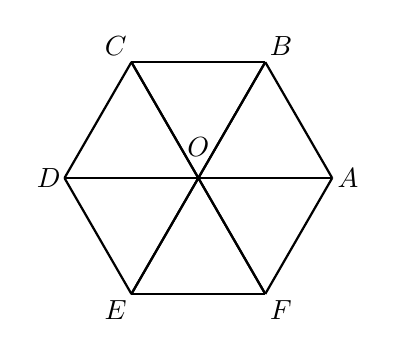
\begin{tikzpicture}[scale=1.7,thick]
			\foreach \x in {0,60,...,300} {
				\draw (\x:1 cm) -- (\x + 60:1 cm);
				\draw (\x:1 cm) -- (\x + 180:1 cm);
			}
			\draw  (0:1 cm) node[shift={(0.2,0)}] {$A$}; \draw  (60:1 cm) node[shift={(0.2,0.2)}] {$B$};
			\draw  (120:1 cm) node[shift={(-0.2,0.2)}] {$C$}; \draw  (180:1 cm) node[shift={(-0.2,0)}] {$D$};
			\draw  (240:1 cm) node[shift={(-0.2,-0.2)}] {$E$}; \draw  (300:1 cm) node[shift={(0.2,-0.2)}] {$F$};
			\draw  (0,0.08 ) node[above] {$O$};
	\end{tikzpicture}}
	\loigiai{
	\begin{enumerate}
		\item[a)] Ta có $VT = \overrightarrow{CD} + \overrightarrow{AO} + \overrightarrow{BA} = \overrightarrow{BA} + \overrightarrow{AO} + \overrightarrow{CD} = \overrightarrow{BO} + \overrightarrow{CD}$.\\
		Do $ABCDEF$ là lục giác đều nên $\overrightarrow{CD} = \overrightarrow{OE}$.\\
		Suy ra $VT = \overrightarrow{BO} + \overrightarrow{OE} = \overrightarrow{BE} = VP$.
		\item[b)] Sắp xếp và gom nhóm các vectơ:
		$$ VT = (\overrightarrow{AB} + \overrightarrow{AF}) + (\overrightarrow{AC} + \overrightarrow{AE}) $$
		Do $ABOF$ là hình bình hành nên $\overrightarrow{AB} + \overrightarrow{AF} = \overrightarrow{AO}$.
		Chèn điểm $D$ vào cụm thứ hai:
		$$ \overrightarrow{AC} + \overrightarrow{AE} = (\overrightarrow{AD} + \overrightarrow{DC}) + (\overrightarrow{AD} + \overrightarrow{DE}) = 2\overrightarrow{AD} + (\overrightarrow{DC} + \overrightarrow{DE}) $$
		Tứ giác $ODEC$ là hình bình hành nên $\overrightarrow{DC} + \overrightarrow{DE} = \overrightarrow{DO} = -\overrightarrow{AO}$.\\
		Do đó: $VT = \overrightarrow{AO} + 2\overrightarrow{AD} - \overrightarrow{AO} = 2\overrightarrow{AD} = VP$.
		\item[c)] Áp dụng tính chất đường trung bình trong các tam giác:
		$$ \overrightarrow{MN} = \dfrac{1}{2}\overrightarrow{AC}; \quad \overrightarrow{PQ} = \dfrac{1}{2}\overrightarrow{CE}; \quad \overrightarrow{RS} = \dfrac{1}{2}\overrightarrow{EA} $$
		Cộng vế theo vế ta được:
		$$ VT = \dfrac{1}{2}(\overrightarrow{AC} + \overrightarrow{CE} + \overrightarrow{EA}) = \dfrac{1}{2}(\overrightarrow{AE} + \overrightarrow{EA}) = \vec{0} = VP. $$
	\end{enumerate}
}
\end{vd} \dongcham{14}

\begin{dang}{Phân tích (biểu diễn) một vectơ theo hai vectơ không cùng phương cho trước}
\end{dang}

\begin{vd}
	Cho tam giác $ABC$. Gọi $M$ là điểm trên cạnh $BC$ sao cho $\overrightarrow{MB}=-3\overrightarrow{MC}$. Phân tích vectơ $\overrightarrow{AM}$ theo $2$ vectơ $\overrightarrow{AB}$ và $\overrightarrow{AC}$.
		\loigiai{
		Ta có $\overrightarrow{MB} = -3\overrightarrow{MC}$. Chèn điểm $A$ vào hai vế bằng quy tắc hiệu, ta được:
		$$ \overrightarrow{AB} - \overrightarrow{AM} = -3(\overrightarrow{AC} - \overrightarrow{AM}) $$
		$$ \Leftrightarrow \overrightarrow{AB} - \overrightarrow{AM} = -3\overrightarrow{AC} + 3\overrightarrow{AM} $$
		$$ \Leftrightarrow 4\overrightarrow{AM} = \overrightarrow{AB} + 3\overrightarrow{AC} \Leftrightarrow \overrightarrow{AM} = \dfrac{1}{4}\overrightarrow{AB} + \dfrac{3}{4}\overrightarrow{AC}. $$
	}
\end{vd} \dongcham{10}

\begin{vd}
	Cho tam giác $ABC$. Gọi $M$ là trung điểm $BC$, $D$ là trung điểm $AM$. Phân tích $\overrightarrow{AD}$ theo 2 vectơ $\overrightarrow{AB}$ và $\overrightarrow{AC}$.
		\loigiai{
		Vì $D$ là trung điểm của $AM$ nên $\overrightarrow{AD} = \dfrac{1}{2}\overrightarrow{AM}$.\\
		Vì $M$ là trung điểm của $BC$ nên $\overrightarrow{AM} = \dfrac{1}{2}(\overrightarrow{AB} + \overrightarrow{AC})$.\\
		Thay vào biểu thức trên, ta được:
		$$ \overrightarrow{AD} = \dfrac{1}{2} \left[ \dfrac{1}{2}(\overrightarrow{AB} + \overrightarrow{AC}) \right] = \dfrac{1}{4}\overrightarrow{AB} + \dfrac{1}{4}\overrightarrow{AC}. $$
	}
\end{vd} \dongcham{10}
\begin{vd}
	Cho hình bình hành $ABCD$ có tâm $O$. Gọi $I$ là trung điểm $BO$. Phân tích vectơ $\overrightarrow{AI}$ theo $\overrightarrow{AB}$ và $\overrightarrow{AD}$.
		\loigiai{
		Vì $I$ là trung điểm của $BO$ nên áp dụng quy tắc trung điểm cho $\triangle ABO$, ta có:
		$$ \overrightarrow{AI} = \dfrac{1}{2}(\overrightarrow{AB} + \overrightarrow{AO}) $$
		Do $O$ là tâm hình bình hành nên $O$ là trung điểm $AC \Rightarrow \overrightarrow{AO} = \dfrac{1}{2}\overrightarrow{AC}$.
		Mặt khác, theo quy tắc hình bình hành $\overrightarrow{AC} = \overrightarrow{AB} + \overrightarrow{AD}$, nên $\overrightarrow{AO} = \dfrac{1}{2}(\overrightarrow{AB} + \overrightarrow{AD})$.\\
		Thay vào biểu thức ban đầu, ta được:
		$$ \overrightarrow{AI} = \dfrac{1}{2}\overrightarrow{AB} + \dfrac{1}{2} \left[ \dfrac{1}{2}(\overrightarrow{AB} + \overrightarrow{AD}) \right] = \dfrac{1}{2}\overrightarrow{AB} + \dfrac{1}{4}\overrightarrow{AB} + \dfrac{1}{4}\overrightarrow{AD} = \dfrac{3}{4}\overrightarrow{AB} + \dfrac{1}{4}\overrightarrow{AD}. $$
	}
\end{vd} \dongcham{12}

\begin{vd}
	Cho tam giác $ABC$ có trọng tâm $G$. Gọi $D$, $E$, $F$ lần lượt là trung điểm của $BC$, $CA$, $AB$ và $I$ là giao điểm của $AD$ và $EF$.
	\begin{tasks}(1)
		\task Hãy phân tích các véc tơ $\overrightarrow{BC},\text{ }\overrightarrow{AI},\text{ }\overrightarrow{AG},\text{ }\overrightarrow{DE},\text{ }\overrightarrow{DC}$ theo $\overrightarrow{AE}$ và $\overrightarrow{AF}$.
		\task Phân tích $\overrightarrow{AB},\text{ }\overrightarrow{AC},\text{ }\overrightarrow{BC,}\text{ }\overrightarrow{GC}$ theo $\overrightarrow{GA}$ và $\overrightarrow{GB}$.
	\end{tasks}
	\loigiai{
	\begin{enumerate}
		\item[a)] Ta nhận thấy $E, F$ là trung điểm $AC, AB$ nên $\overrightarrow{AC} = 2\overrightarrow{AE}$ và $\overrightarrow{AB} = 2\overrightarrow{AF}$.
		\begin{itemize}
			\item $\overrightarrow{BC} = \overrightarrow{AC} - \overrightarrow{AB} = 2\overrightarrow{AE} - 2\overrightarrow{AF}$.
			\item Do $D$ là trung điểm $BC$, $\overrightarrow{AD} = \dfrac{1}{2}(\overrightarrow{AB} + \overrightarrow{AC}) = \dfrac{1}{2}(2\overrightarrow{AF} + 2\overrightarrow{AE}) = \overrightarrow{AF} + \overrightarrow{AE}$.\\
			$EF$ là đường trung bình, cắt trung tuyến $AD$ tại $I$ nên $I$ là trung điểm $AD$.\\
			Suy ra $\overrightarrow{AI} = \dfrac{1}{2}\overrightarrow{AD} = \dfrac{1}{2}\overrightarrow{AE} + \dfrac{1}{2}\overrightarrow{AF}$.
			\item Vì $G$ là trọng tâm nên $\overrightarrow{AG} = \dfrac{2}{3}\overrightarrow{AD} = \dfrac{2}{3}(\overrightarrow{AE} + \overrightarrow{AF}) = \dfrac{2}{3}\overrightarrow{AE} + \dfrac{2}{3}\overrightarrow{AF}$.
			\item $\overrightarrow{DE} = \overrightarrow{AE} - \overrightarrow{AD} = \overrightarrow{AE} - (\overrightarrow{AE} + \overrightarrow{AF}) = -\overrightarrow{AF}$.
			\item $\overrightarrow{DC} = \dfrac{1}{2}\overrightarrow{BC} = \dfrac{1}{2}(2\overrightarrow{AE} - 2\overrightarrow{AF}) = \overrightarrow{AE} - \overrightarrow{AF}$.
		\end{itemize}
		\item[b)] Dựa vào tính chất trọng tâm $\overrightarrow{GA} + \overrightarrow{GB} + \overrightarrow{GC} = \vec{0} \Rightarrow \overrightarrow{GC} = -\overrightarrow{GA} - \overrightarrow{GB}$.
		\begin{itemize}
			\item $\overrightarrow{AB} = \overrightarrow{GB} - \overrightarrow{GA} = -\overrightarrow{GA} + \overrightarrow{GB}$.
			\item $\overrightarrow{AC} = \overrightarrow{GC} - \overrightarrow{GA} = (-\overrightarrow{GA} - \overrightarrow{GB}) - \overrightarrow{GA} = -2\overrightarrow{GA} - \overrightarrow{GB}$.
			\item $\overrightarrow{BC} = \overrightarrow{GC} - \overrightarrow{GB} = (-\overrightarrow{GA} - \overrightarrow{GB}) - \overrightarrow{GB} = -\overrightarrow{GA} - 2\overrightarrow{GB}$.
		\end{itemize}
	\end{enumerate}
}
\end{vd} \dongcham{18}

\begin{vd}
	Cho tam giác $ABC$. Gọi $M$ là trung điểm cạnh $AB$ và $N$ là điểm trên đoạn $AC$ sao cho $NA = 2NC$, $K$ là trung điểm của $MN$.
	\begin{tasks}(2)
		\task Phân tích $\overrightarrow{AK}$ theo 2 véc tơ $\overrightarrow{AB}$ và $\overrightarrow{AC}$.
		\task Chứng minh $\overrightarrow{AC}+\dfrac{3}{2}\overrightarrow{BN}+3\overrightarrow{NM}=\overrightarrow{0}$.
	\end{tasks}
	\loigiai{
	\begin{enumerate}
		\item[a)] Vì $M$ là trung điểm $AB$ nên $\overrightarrow{AM} = \dfrac{1}{2}\overrightarrow{AB}$.\\
		Vì $N$ thuộc đoạn $AC$ và $NA = 2NC$ nên $AN = \dfrac{2}{3}AC \Rightarrow \overrightarrow{AN} = \dfrac{2}{3}\overrightarrow{AC}$.\\
		Vì $K$ là trung điểm của $MN$ nên:
		$$ \overrightarrow{AK} = \dfrac{1}{2}(\overrightarrow{AM} + \overrightarrow{AN}) = \dfrac{1}{2} \left( \dfrac{1}{2}\overrightarrow{AB} + \dfrac{2}{3}\overrightarrow{AC} \right) = \dfrac{1}{4}\overrightarrow{AB} + \dfrac{1}{3}\overrightarrow{AC}. $$
		
		\item[b)] Ta biến đổi vế trái của đẳng thức:
		$$ VT = \overrightarrow{AC} + \dfrac{3}{2}\overrightarrow{BN} + 3\overrightarrow{NM} = \overrightarrow{AC} + \dfrac{3}{2}(\overrightarrow{AN} - \overrightarrow{AB}) + 3(\overrightarrow{AM} - \overrightarrow{AN}) $$
		$$ = \overrightarrow{AC} + \dfrac{3}{2}\overrightarrow{AN} - \dfrac{3}{2}\overrightarrow{AB} + 3\overrightarrow{AM} - 3\overrightarrow{AN} = \overrightarrow{AC} - \dfrac{3}{2}\overrightarrow{AN} - \dfrac{3}{2}\overrightarrow{AB} + 3\overrightarrow{AM} $$
		Thay $\overrightarrow{AN} = \dfrac{2}{3}\overrightarrow{AC}$ và $\overrightarrow{AM} = \dfrac{1}{2}\overrightarrow{AB}$ vào biểu thức:
		$$ VT = \overrightarrow{AC} - \dfrac{3}{2} \left( \dfrac{2}{3}\overrightarrow{AC} \right) - \dfrac{3}{2}\overrightarrow{AB} + 3 \left( \dfrac{1}{2}\overrightarrow{AB} \right) $$
		$$ VT = \overrightarrow{AC} - \overrightarrow{AC} - \dfrac{3}{2}\overrightarrow{AB} + \dfrac{3}{2}\overrightarrow{AB} = \vec{0} = VP \text{ (điều phải chứng minh)}. $$
	\end{enumerate}
}
\end{vd} \dongcham{15}
\begin{dang}{Tìm điều kiện hoặc chứng minh tính chất song song, thẳng hàng}
	
\end{dang}

\begin{vd}%[0H1B3-5]
	Cho $\triangle ABC$ có $M$ là trung điểm của cạnh $BC$. Các điểm $D$, $E$ thỏa mãn đẳng thức $\overrightarrow{BD}= 4 \overrightarrow{BA}$, $\overrightarrow{AE}= 3 \overrightarrow{AC}$. Chứng minh $DE \parallel AM$.
	\loigiai{
		\immini
		{
			Ta có $M$ là trung điểm của $BC$ nên $\overrightarrow{AM}= \dfrac{1}{2}\left( \overrightarrow{AB}+ \overrightarrow{AC}\right)$.\\
			Vì $\overrightarrow{BD}= 4 \overrightarrow{BA} \Rightarrow \overrightarrow{AD}= -3\overrightarrow{AB}$. Do đó\\
			$\overrightarrow{DE}= \overrightarrow{AE}- \overrightarrow{AD}= 3 \overrightarrow{AC} + 3\overrightarrow{AB}= 6 \overrightarrow{AM}$.\\
			Suy ra hai véc-tơ $\overrightarrow{DE}$ và $\overrightarrow{AM}$ cùng phương. Vậy $DE \parallel AM$.
		}
		{
			\begin{tikzpicture}[scale=.7, font=\footnotesize, line join=round, line cap=round, >=stealth]
				\coordinate (A) at (0,0);
				\coordinate (B) at (-.5,-1);
				\coordinate (C) at (1.5,-1);
				\coordinate (M) at ($(B)!.5!(C)$);
				\coordinate (D) at ($(B)!4!(A)$);
				\coordinate (E) at ($(A)!3!(C)$);
				\draw (B)--(D)--(E)--(A)--(M) (B)--(C);
				\foreach \p/\pos in {A/above left, B/below, C/below, D/above, M/below, E/below}
				\fill (\p) circle (1pt) node[\pos] {$\p$};
			\end{tikzpicture}
		}
	}
\end{vd} \dongcham{14}

\begin{vd}%[0H1B3-5]
	Cho bốn điểm phân biệt $A$, $B$, $C$, $D$ thỏa: $2\overrightarrow{AB} + 3\overrightarrow{AC}=5\overrightarrow{AD}$. Chứng minh $B$, $C$, $D$ thẳng hàng.
	\loigiai{
		Ta có
		\begin{eqnarray*}
			& & 2\overrightarrow{AB} + 3\overrightarrow{AC}=5\overrightarrow{AD}\\
			&\Leftrightarrow& 2\overrightarrow{AB} + 3\overrightarrow{AC}-5\overrightarrow{AD}=\overrightarrow{0}\\
			&\Leftrightarrow& 2\overrightarrow{AB} -2\overrightarrow{AD}+ 3\overrightarrow{AC}-3\overrightarrow{AD}=\overrightarrow{0}\\
			&\Leftrightarrow& 2\left(\overrightarrow{AB} - \overrightarrow{AD}\right)+3\left(\overrightarrow{AC} - \overrightarrow{AD}\right)=\overrightarrow{0}\\
			&\Leftrightarrow& 2\overrightarrow{DB}+3\overrightarrow{DC}=\overrightarrow{0}\\
			&\Leftrightarrow& \overrightarrow{DB} = -\dfrac{3}{2}\overrightarrow{DC}.
		\end{eqnarray*}
		Suy ra ba điểm $B$, $C$, $D$ thẳng hàng.
	}
\end{vd} \dongcham{20}

\begin{vd}
	Cho hình bình hành $ABCD$ có $G$ là trọng tâm $\Delta BMN$. Gọi $M$, $N$ là điểm sao cho $\overrightarrow{MB}=-2\overrightarrow{MA}$, $\overrightarrow{ND}=\dfrac{1}{2}\overrightarrow{CD}$.
	\begin{tasks}(1)
		\task Phân tích $\overrightarrow{AN},\text{ }\overrightarrow{AG}$ theo 2 vectơ $\overrightarrow{a}=\overrightarrow{AB}$ và  $\overrightarrow{b}=\overrightarrow{AC}$.
		\task Gọi $I$ là điểm trên $BC$ sao cho $\overrightarrow{BI}=k\overrightarrow{BC}$ Tìm $k$ để $A$, $G$, $I$ thẳng hàng.
	\end{tasks}
	\loigiai{
	\begin{enumerate}
		\item[a)] Theo quy tắc hình bình hành ta có $\overrightarrow{AD} = \overrightarrow{AC} - \overrightarrow{AB} = \vec{b} - \vec{a}$.\\
		Từ giả thiết $\overrightarrow{ND} = \dfrac{1}{2}\overrightarrow{CD} \Rightarrow \overrightarrow{DN} = -\dfrac{1}{2}\overrightarrow{CD} = \dfrac{1}{2}\overrightarrow{DC} = \dfrac{1}{2}\overrightarrow{AB} = \dfrac{1}{2}\vec{a}$.\\
		Ta có: $\overrightarrow{AN} = \overrightarrow{AD} + \overrightarrow{DN} = (\vec{b} - \vec{a}) + \dfrac{1}{2}\vec{a} = -\dfrac{1}{2}\vec{a} + \vec{b}$.\\
		Mặt khác, $\overrightarrow{MB} = -2\overrightarrow{MA} \Leftrightarrow \overrightarrow{AM} = \dfrac{1}{3}\overrightarrow{AB} = \dfrac{1}{3}\vec{a}$.\\
		Vì $G$ là trọng tâm $\triangle BMN$ nên:
		$$ \overrightarrow{AG} = \dfrac{1}{3}(\overrightarrow{AB} + \overrightarrow{AM} + \overrightarrow{AN}) $$
		$$ = \dfrac{1}{3} \left( \vec{a} + \dfrac{1}{3}\vec{a} - \dfrac{1}{2}\vec{a} + \vec{b} \right) = \dfrac{1}{3} \left( \dfrac{5}{6}\vec{a} + \vec{b} \right) = \dfrac{5}{18}\vec{a} + \dfrac{1}{3}\vec{b}. $$
		
		\item[b)] Ta có: $\overrightarrow{AI} = \overrightarrow{AB} + \overrightarrow{BI} = \overrightarrow{AB} + k\overrightarrow{BC}$.\\
		Vì $ABCD$ là hình bình hành nên $\overrightarrow{BC} = \overrightarrow{AD} = \vec{b} - \vec{a}$.\\
		Suy ra: $\overrightarrow{AI} = \vec{a} + k(\vec{b} - \vec{a}) = (1 - k)\vec{a} + k\vec{b}$.\\
		Để ba điểm $A, G, I$ thẳng hàng thì phải tồn tại số thực $m$ sao cho $\overrightarrow{AI} = m\overrightarrow{AG}$.
		$$ \Rightarrow (1 - k)\vec{a} + k\vec{b} = m \left( \dfrac{5}{18}\vec{a} + \dfrac{1}{3}\vec{b} \right) \Leftrightarrow (1 - k)\vec{a} + k\vec{b} = \dfrac{5m}{18}\vec{a} + \dfrac{m}{3}\vec{b}. $$
		Vì $\vec{a}, \vec{b}$ là hai vectơ không cùng phương nên ta có hệ phương trình:
		$$ \heva{1 - k &= \dfrac{5m}{18} \\ k &= \dfrac{m}{3}} \Leftrightarrow \heva{1 - k &= \dfrac{5}{18} \cdot 3k \\ m &= 3k} \Leftrightarrow \heva{1 &= \dfrac{15k}{18} + k \\ m &= 3k} \Leftrightarrow \heva{1 &= \dfrac{11k}{6} \\ m &= 3k} \Leftrightarrow \heva{k &= \dfrac{6}{11} \\ m &= \dfrac{18}{11}} $$
		Vậy $k = \dfrac{6}{11}$ thì $A, G, I$ thẳng hàng.
	\end{enumerate}
}
\end{vd} \dongcham{17}

\begin{dang}{Xác định điểm thỏa mãn một đẳng thức vectơ cho trước}
	
\end{dang}

\begin{vd}
	Cho tam giác $ABC$. Hãy xác định các điểm $I$, $J$, $K$, $L$ thoả các đẳng thức sau
	\begin{tasks}(2)
		\task $2\overrightarrow{IA}-3\overrightarrow{IB}=3\overrightarrow{BC}$.
		\task $\overrightarrow{JA}+\overrightarrow{JB}+2\overrightarrow{JC}=\overrightarrow{0}$.
		\task $\overrightarrow{KA}+\overrightarrow{KB}-\overrightarrow{KC}=\overrightarrow{BC}$.
		\task $\overrightarrow{LA}-2\overrightarrow{LC}=\overrightarrow{AB}-2\overrightarrow{AC}$.
	\end{tasks}
	\loigiai{
	\begin{enumerate}
		\item[a)] Chèn điểm $A$ vào $\overrightarrow{IB}$, ta có: $2\overrightarrow{IA} - 3(\overrightarrow{IA} + \overrightarrow{AB}) = 3\overrightarrow{BC}$
		$$ \Leftrightarrow -\overrightarrow{IA} - 3\overrightarrow{AB} = 3\overrightarrow{BC} \Leftrightarrow \overrightarrow{AI} = 3\overrightarrow{AB} + 3\overrightarrow{BC} = 3(\overrightarrow{AB} + \overrightarrow{BC}) = 3\overrightarrow{AC}. $$
		Vậy điểm $I$ nằm trên tia $AC$ sao cho độ dài $AI = 3AC$.
		
		\item[b)] Gọi $M$ là trung điểm của $AB$, theo tính chất trung điểm ta có $\overrightarrow{JA} + \overrightarrow{JB} = 2\overrightarrow{JM}$.
		Thay vào đẳng thức ban đầu:
		$$ 2\overrightarrow{JM} + 2\overrightarrow{JC} = \vec{0} \Leftrightarrow \overrightarrow{JM} + \overrightarrow{JC} = \vec{0}. $$
		Vậy $J$ là trung điểm của đoạn thẳng $MC$ (với $M$ là trung điểm cạnh $AB$).
		
		\item[c)] Ghép cặp và áp dụng quy tắc trừ: $\overrightarrow{KA} + (\overrightarrow{KB} - \overrightarrow{KC}) = \overrightarrow{BC}$
		$$ \Leftrightarrow \overrightarrow{KA} + \overrightarrow{CB} = \overrightarrow{BC} \Leftrightarrow \overrightarrow{KA} = \overrightarrow{BC} - \overrightarrow{CB} = \overrightarrow{BC} + \overrightarrow{BC} = 2\overrightarrow{BC}. $$
		$$ \Leftrightarrow \overrightarrow{AK} = 2\overrightarrow{CB}. $$
		Vậy điểm $K$ được xác định sao cho $\overrightarrow{AK}$ cùng hướng với $\overrightarrow{CB}$ và có độ dài $AK = 2BC$.
		
		\item[d)] Chèn điểm $A$ vào $\overrightarrow{LC}$, ta có: $\overrightarrow{LA} - 2(\overrightarrow{LA} + \overrightarrow{AC}) = \overrightarrow{AB} - 2\overrightarrow{AC}$
		$$ \Leftrightarrow -\overrightarrow{LA} - 2\overrightarrow{AC} = \overrightarrow{AB} - 2\overrightarrow{AC} $$
		$$ \Leftrightarrow \overrightarrow{AL} = \overrightarrow{AB}. $$
		Hai vectơ có chung điểm gốc $A$ và bằng nhau nên hai điểm ngọn trùng nhau. Vậy điểm $L$ trùng với điểm $B$ ($L \equiv B$).
	\end{enumerate}
}
\end{vd} \dongcham{12}

\boxmini{BÀI TẬP TỔNG HỢP TỰ LUYỆN}
\begin{baitap}%[Tex hóa SGK CD-CT,T7/22, Trần Nhân Kiệt]%[0H1B3-1]
	\immini{
		Cho hai véc-tơ $\vec{a}$, $\vec{b}$ và một điểm $M$ như hình bên
		\begin{enumEX}{1}
			\item Hãy vẽ các véc-tơ $\vec{MN}=2\vec{a}$, $\vec{MP}=-2\vec{b}$.
			\item Cho biết mỗi ô vuông có cạnh bằng $1$. Tính $\left|5\vec{a}\right|$, $\left|-5\vec{b}\right|$.
		\end{enumEX}
	}
	{
		\begin{tikzpicture}[scale=1, font=\footnotesize, line join=round, line cap=round, >=stealth]
			\path 	(0:0) coordinate (M);
			\draw[->,very thick] (-2,0)--(-1,1) node[below right=1pt]{$\vec{b}$};
			\draw[->,very thick] (-1,1) -- (1,1)node[above left=2pt]{$\vec{a}$};
			\draw[step=1cm,very thin] (-3,-1) grid (2,2);
			\foreach \x/\g in {M/-40}
			\fill[black] 	(\x) circle (1pt)
			($(\g:4mm)+(\x)$) node {$\x$};	
			
		\end{tikzpicture}
	}
	\loigiai{
		\immini{
			\begin{enumEX}{1}
				\item Điểm $M$, $P$ như hình vẽ.
				\item Ta có\\
				$|5\vec{a}|=5|\vec{a}|=5\cdot 2=10$ và\\
				$\left|-5\vec{b}\right|=|-5|\cdot \left|\vec{b}\right|=5\sqrt{2}$.
			\end{enumEX}
		}
		{
			\begin{tikzpicture}[scale=1, font=\footnotesize, line join=round, line cap=round, >=stealth]
				\path 	(0:0) coordinate (M)
				++(0:4) coordinate (N);
				\draw[->,very thick] (-2,0)--(-1,1) node[below right=2pt]{$\vec{b}$};
				\draw[->,very thick] (-1,1) -- (1,1)node[above left=2pt]{$\vec{a}$};
				\draw[->,very thick] (0,0) -- (-2,-2)node[above left=2pt]{$P$};
				\draw[step=1cm,very thin] (-3,-3) grid (5,2);
				\draw[->,very thick] (M)--(N);
				\draw (-1.1,-1) node[below right=1pt]{$-2\vec{b}$};
				\draw (2.4,.6) node[below=1pt]{$2\vec{a}$};
				\foreach \x/\g in {M/-40,N/-90}
				\fill[black] 	(\x) circle (1pt)
				($(\g:4mm)+(\x)$) node {$\x$};	
				
			\end{tikzpicture}
		}
	}
\end{baitap}

\begin{baitap}%[Tex hóa SGK CD-CT,T7/22, Trần Nhân Kiệt]%[0H1B3-2]
	Lấy một điểm $M$ tuỳ ý. Chứng minh rằng
	\begin{enumEX}{1}
		\item $I$ là trung điểm của đoạn thẳng $AB$ khi và chỉ khi $\vec{MA}+\vec{MB}=2\vec{MI}$.
		\item $G$ là trọng tâm của tam giác $ABC$ khi và chỉ khi $\vec{MA}+\vec{MB}+\vec{MC}=3\vec{MG}$.
	\end{enumEX}
	\loigiai{
		\begin{enumEX}{1}
			\item $I$ là trung điểm của đoạn thẳng $AB$ khi và chỉ khi $\vec{IA}+\vec{IB}=\vec{0}$
			\begin{eqnarray*}
				&\Leftrightarrow& \left(\vec{IM}+\vec{MA}\right)+\left(\vec{IM}+\vec{MB}\right)=\vec{0}\\
				&\Leftrightarrow& 2\vec{MI}+\vec{MA}+\vec{MB}=\vec{0}\\
				&\Leftrightarrow&\vec{MA}+\vec{MB}=2\vec{MI}.
			\end{eqnarray*}
			\item $G$ là trọng tâm của tam giác $ABC$ khi và chỉ khi $\vec{GA}+\vec{GB}+\vec{GC}=\vec{0}$
			\begin{eqnarray*}
				&\Leftrightarrow& \left(\vec{GM}+\vec{MA}\right)+\left(\vec{GM}+\vec{MB}\right)+\left(\vec{GM}+\vec{MC}\right)=\vec{0}\\
				&\Leftrightarrow& 3\vec{GM}+\vec{GA}+\vec{GB}+\vec{GC}=\vec{0}\\
				&\Leftrightarrow& \vec{MA}+\vec{MB}+\vec{MC}=3\vec{MG}.
			\end{eqnarray*}
		\end{enumEX}
	}
\end{baitap}

\begin{baitap}%[Tex hóa SGK CD-CT,T7/22, Trần Nhân Kiệt]%[0H1B3-3]
	Cho hai điểm phân biệt $A$ và $B$. Tìm điểm $K$ sao cho $3\vec{KA}+2\vec{KB}=\vec{0}$.
	\loigiai{
		\immini{
			Ta có
			\begin{eqnarray*}
				&&3\vec{KA}+2\vec{KB}=\vec{0}\\
				&\Leftrightarrow& 3\vec{KA}+2\left(\vec{KA}+\vec{AB}\right)=\vec{0}\\
				&\Leftrightarrow& 5\vec{KA}+2\vec{AB}=\vec{0}\\
				&\Leftrightarrow& \vec{AK}=\dfrac{2}{5}\vec{AB}.
			\end{eqnarray*}
		}
		{
			\begin{tikzpicture}[scale=1, font=\footnotesize, line join=round, line cap=round, >=stealth]
				\path 	(0:0) coordinate (A)
				++(0:4) coordinate (B);
				\coordinate (K) at ($(A)!2/5!(B)$);
				\draw[] 	(A)--(B);
				\foreach \x/\g in {A/90,B/90,K/90}
				\fill[black] 	(\x) circle (1pt)
				($(\g:3mm)+(\x)$) node {$\x$};	
				
			\end{tikzpicture}
		}
	}
\end{baitap}

\begin{baitap}%[0H1K3-2]%
	Cho tam giác $ABC$ có $G$ là trọng tâm tam giác và $I$ là điểm đối xứng của $B$ qua $G$, $M$ là trung điểm của $BC$. Chứng minh rằng:
	\begin{listEX}[3]
		\item $2\overrightarrow{AC}-\overrightarrow{AB}=3\overrightarrow{AI}$.
		\item $2\overrightarrow{AB}+3\overrightarrow{AC}=6\overrightarrow{IC}$.
		\item $\overrightarrow{AC}-5\overrightarrow{AB}=6\overrightarrow{MI}$.
	\end{listEX}
	\loigiai{
		
		\begin{listEX}[1]
			\item Vì $G$ là trọng tâm tam giác $ABC$ nên $2\overrightarrow{GM}=\overrightarrow{AG}$. $I$ đối xứng của điểm $B$ qua $G$ nên $\overrightarrow{BG}=\overrightarrow{GI}$.
			\immini
			{Gọi $N$ là trung điểm $AC$, khi đó $AM=MC$, $GM =MI$ hay tứ giác $AGCI$ là hình bình hành, suy ra $\overrightarrow{AI}=\overrightarrow{GC}$.\\
				Ta có $2\overrightarrow{AC} -\overrightarrow{AB}=2\left(\overrightarrow{AI}+\overrightarrow{IC}\right) -\left(\overrightarrow{AI}+\overrightarrow{IB}\right) = \overrightarrow{AI}+2\overrightarrow{IC}-\overrightarrow{IB}=\overrightarrow{IA}+2\overrightarrow{IC}-2\overrightarrow{IG}=\overrightarrow{IA}-2\overrightarrow{GC}=\overrightarrow{IA}+2\overrightarrow{AI}=3\overrightarrow{AI}$.
			}
			{\begin{tikzpicture}[scale=1, font=\footnotesize, line join=round, line cap=round,fill=black, >=stealth]%[fill=black]
					\coordinate (A) at (0,0);
					\coordinate (B) at (2,3);
					\coordinate (C) at (5,0);
					\coordinate (M) at ($(B)!0.5!(C)$);
					\coordinate (G) at ($(A)!0.66!(M)$);
					\coordinate (I) at ($2*(G)-(B)$);
					\tkzLabelPoints[above](B)
					\tkzLabelPoints[below](A,C,I)
					\tkzLabelPoints[right](M,G)
					\tkzDrawPoints(A,B,C,M,I,G)
					\tkzDrawSegments (A,B B,C C,A B,I A,M)
			\end{tikzpicture}}
			\item $2\overrightarrow{AB}+3\overrightarrow{AC}=6\overrightarrow{IC}$.
			\item $\overrightarrow{AC}-5\overrightarrow{AB}=6\overrightarrow{MI}$.
		\end{listEX}
	}
\end{baitap} \cham{20}

\begin{baitap}
	Cho hình bình hành $ABCD$ tâm $O$. Gọi $M$, $N$ theo thứ tự là trung điểm của $AB$, $CD$ và $P$ là điểm thỏa mãn hệ thức $\overrightarrow{OP} = - \dfrac{1}{3} \overrightarrow{OA}$.
	\begin{enumerate}
		\item Chứng minh rằng $3 \overrightarrow{AP} - 2 \overrightarrow{AC} = \overrightarrow{0}$
		\item Chứng minh $3$ điểm $B$, $P$, $N$ thẳng hàng.
		\item Chứng minh $3$ đường $AC$, $BD$ và $MN$ đồng quy.
	\end{enumerate}
	\loigiai{
		\begin{enumerate}
			\item \immini{Ta có $\overrightarrow{OP} = - \dfrac{1}{3} \overrightarrow{OA} \Leftrightarrow 3 \overrightarrow{OP} = - \overrightarrow{OA} $ \\ $ \Leftrightarrow 3 \left( \overrightarrow{OA} + \overrightarrow{AP} \right) = - \overrightarrow{OA} \Leftrightarrow 4 \overrightarrow{OA} + 3 \overrightarrow{AP} = \overrightarrow{0} $. \hfill(1)\\
				Do $O$ là trung điểm của $AC$ nên $\overrightarrow{OA} = - \dfrac{1}{2} \overrightarrow{AC}$, thay vào $(1)$ ta được\\ $3 \overrightarrow{AP} - 2 \overrightarrow{AC} = \overrightarrow{0}$ (đpcm).}{
				
				\begin{tikzpicture}[scale=.8]
					\tkzDefPoints{0/0/A, -1/-2/D, 4/-2/C}
					\coordinate (B) at ($(A)+(C)-(D)$);
					\coordinate (O) at ($(A)!.5!(C)$);
					\coordinate (M) at ($(A)!.5!(B)$);
					\coordinate (N) at ($(D)!.5!(C)$);
					\coordinate (P) at ($(O)!.33!(C)$);
					\draw (2.2,-1) node[above left]{$O$} ;
					\tkzDrawSegments[dashed](M,N B,N)
					\tkzDrawPolygon(A,D,B)
					\tkzDrawSegments(A,C D,C C,B)
					\tkzLabelPoints[left](A)
					\tkzLabelPoints[above](M,B)
					\tkzLabelPoints[below](N,D,C,P)
					\tkzDrawPoints(A,B,C,D,M,N,P,O)
			\end{tikzpicture}}
			
			\item Để chứng minh $B$, $P$, $N$ thẳng hàng ta chứng minh $\overrightarrow{BP}$ cùng phương với $\overrightarrow{BN}$.
			\begin{itemize}
				\item Tính $\overrightarrow{BP} $ theo $\overrightarrow{BA}$, $\overrightarrow{BC}$.\\
				Ta có $\overrightarrow{BP} = \overrightarrow{BA} + \overrightarrow{AP}$, mà $\overrightarrow{AP} = \dfrac{2}{3} \Rightarrow \overrightarrow{BP} = \overrightarrow{BA} + \dfrac{2}{3} \overrightarrow{AC}$. \hfill(2)\\
				Do $ABCD$ là hình bình hành nên $\overrightarrow{AC} = \overrightarrow{AB} + \overrightarrow{AD} = \overrightarrow{AB} + \overrightarrow{BC}$, thay vào $(2)$ ta được
				\begin{align}
					\overrightarrow{BP} = \overrightarrow{BA} + \dfrac{2}{3} \overrightarrow{AB} + \dfrac{2}{3} \overrightarrow{BC} = \dfrac{1}{3} \overrightarrow{BA} + \dfrac{2}{3} \overrightarrow{BC} \Rightarrow 3 \overrightarrow{BP} = \overrightarrow{BA} + 2 \overrightarrow{BC}. \tag{3}
				\end{align}
				\item Tính $\overrightarrow{BN} $ theo $\overrightarrow{BA}$, $\overrightarrow{BC}$. Ta có
				\begin{align}
					\overrightarrow{BN} &= \dfrac{1}{2} \left( \overrightarrow{BD} + \overrightarrow{BC} \right) = \dfrac{1}{2} \overrightarrow{BD} + \dfrac{1}{2}  \overrightarrow{BC} \notag\\ &= \dfrac{1}{2} \left( \overrightarrow{BA}+ \overrightarrow{BC} \right) + \dfrac{1}{2} \overrightarrow{BC} = \overrightarrow{BC}+ \dfrac{1}{2} \overrightarrow{BA}. \notag \\
					&\Rightarrow  2 \overrightarrow{BN} = \overrightarrow{BA} + 2 \overrightarrow{BC}. \tag{4}
				\end{align}
			\end{itemize}
			Từ $(3)$ và $(4)$ ta có $3 \overrightarrow{BP} = 2 \overrightarrow{BN} \Rightarrow \overrightarrow{BP} = \dfrac{2}{3} \overrightarrow{BN}$, suy ra $P$, $B$, $N$ thẳng hàng.
			
			\item Giả sử $AC \cap BD = O$, ta chứng minh $O \in MN$. Thật vậy
			\begin{itemize}
				\item Vì $MO$ là đường trung bình của tam giác $\triangle ABD$ nên $\overrightarrow{OM} = \dfrac{1}{2} \overrightarrow{DA}$.
				\item Vì $ON$ là đường trung bình của tam giác $\triangle ACB$ nên $\overrightarrow{ON} = \dfrac{1}{2} \overrightarrow{BC} = - \dfrac{1}{2} \overrightarrow{DA}$.
			\end{itemize}
			Do đó ta có $\overrightarrow{OM}+ \overrightarrow{ON} = \overrightarrow{0}$. Hay $O$ là trung điểm của $MN$, suy ra $O$ cùng thuộc $3$ đường $AC$, $BD$, $MN$ hay $3$ đường $AC$, $BD$ và $MN$ đồng quy.
		\end{enumerate}
	}
\end{baitap} \cham{32}



